% 2006 天津文科 Q13，源：固定 PDF 第 1 页（印刷页 338）。
% 识别映射：实棱 AB, BC, AA_1, BB_1, CC_1, A_1B_1, B_1C_1, C_1A_1, BC_1；
% 虚棱 AC；虚线段 AC_1。节点为 A,B,C,A_1,B_1,C_1。原图中 AC 与 AC_1 均为虚线。
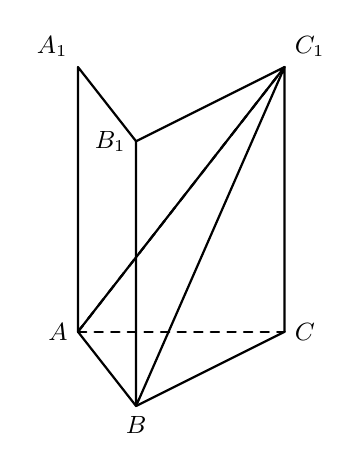
\begin{tikzpicture}[x=0.82cm,y=0.82cm,line cap=round,line join=round,line width=0.8pt,font=\small]
  \coordinate (A) at (0,0);
  \coordinate (B) at (0.9,-1.15);
  \coordinate (C) at (3.2,0);
  \coordinate (A1) at (0,4.1);
  \coordinate (B1) at (0.9,2.95);
  \coordinate (C1) at (3.2,4.1);
  \draw[dashed] (A)--(C);
  \draw[dashed] (A)--(C1);
  \draw (A)--(B)--(C);
  \draw (A)--(A1)--(B1)--(C1)--cycle;
  \draw (B)--(B1) (C)--(C1) (B)--(C1);
  \node[left] at (A) {$A$};
  \node[below] at (B) {$B$};
  \node[right] at (C) {$C$};
  \node[above left] at (A1) {$A_1$};
  \node[left] at (B1) {$B_1$};
  \node[above right] at (C1) {$C_1$};
\end{tikzpicture}
